% =====================================================================
%  4. DESCRIPCIÓN DE LA UNIDAD MINERA
%  Responsable: INTEGRANTE 2
%  ESTADO: REDACTADO (1 de agosto de 2026) — ~3.900 palabras
%  Fuente principal: Sección B de docs/bitacora_decisiones.md
%
%  Contiene la Tabla de reservas y leyes y la Tabla de capacidad de
%  tratamiento. Faltan por insertar la Figura 1 (mapa de ubicación) y la
%  Figura 2 (diagrama de flujo del proceso): los entornos están listos y
%  comentados, solo hay que colocar los archivos en imagenes/.
%
%  ############ LAS CUATRO ADVERTENCIAS DE DATOS ESTÁN RESUELTAS ##########
%  1) Capacidad de planta -> presentada como rango con su fuente en la
%     sección 4.7 y en su tabla, NO como cifra única.
%  2) Las ~24.282 t/día del NI 43-101 -> declaradas expresamente como
%     material total minado (mineral + desmonte), no capacidad de planta.
%  3) Mina Constancia (Perú) -> no se ha tomado ningún dato de esa
%     operación. Si alguien añade cifras nuevas, verificar la fuente.
%  4) Presa de relaves -> tipo, altura y volumen NO verificados en fuente
%     primaria de Marlin; se consigna como limitación de información en
%     la sección 4.9. NO rellenar esos datos sin el EIA detallado o el
%     informe de diseño de Knight Piésold.
%  ######################################################################
% =====================================================================

\section{Descripción de la unidad minera}
\label{sec:unidad}

La caracterización de la unidad minera no es un trámite descriptivo previo al
análisis de la auditoría, sino parte del análisis mismo. Los hallazgos que se
examinan en la sección \ref{sec:hallazgos} solo resultan inteligibles si antes se
comprende qué se extraía, con qué método, mediante qué procesos químicos, sobre
qué territorio y en convivencia con qué población. El uso de cianuro explica la
preocupación por la calidad del agua; el método mixto de explotación explica las
denuncias por agrietamiento de viviendas; la condición indígena del territorio
explica la exigencia de consulta previa; y la magnitud económica de la operación
explica tanto la intensidad del conflicto como la presión internacional que
terminó desembocando en la propia auditoría. Esta sección aporta, por tanto, las
premisas fácticas del resto del informe.

% ---------------------------------------------------------------------
\subsection{Identificación y evolución de la titularidad}

La operación analizada corresponde a la Mina Marlin, también denominada Proyecto
Marlin en la documentación técnica y financiera. Su titular directo fue
\titular, sociedad guatemalteca constituida el 6 de agosto de 1996. La matriz
corporativa durante la mayor parte de la vida útil fue Goldcorp Inc., empresa con
sede en Vancouver, Canadá; tras la fusión societaria de 2019, los activos
históricos de Goldcorp pasaron a integrarse en Newmont
\parencite{sec2011ni43101, goldcorp2023marlin}.

La cadena de titularidad tiene relevancia auditora directa, porque las
obligaciones asumidas en una etapa fueron heredadas por operadores distintos de
quienes las contrajeron. El yacimiento fue descubierto en 1998 por Montana
Exploradora. En 2000 la propiedad fue adquirida por Francisco Gold, compañía que
en 2002 se fusionó con Glamis Gold. Fue Glamis quien obtuvo del Ministerio de
Energía y Minas de Guatemala la licencia de explotación, otorgada el 27 de
noviembre de 2003, y quien gestionó el financiamiento internacional del proyecto.
La construcción se desarrolló entre 2004 y 2005, y la producción de oro y plata
se inició hacia finales de 2005. En 2006 Goldcorp adquirió Glamis Gold e incorporó
la operación a su portafolio. La producción cesó definitivamente el 31 de mayo de
2017 \parencite{sec2011ni43101, prensalibre2017cierre, goldcorp2023marlin}.

Un elemento decisivo de esta etapa inicial es el financiamiento. La Corporación
Financiera Internacional otorgó al proyecto un préstamo de US\$ 45 millones,
decisión que activó la aplicación de sus políticas de salvaguarda ambiental y
social \parencite{ifcsfmarlin}. Esta circunstancia, aparentemente administrativa,
es la que hace jurídicamente pertinentes los IFC Performance Standards expuestos
en la sección \ref{sec:marco} y la que abrió, años más tarde, la vía de la
denuncia ante la Compliance Advisor Ombudsman que se examina en la sección
\ref{sec:critico} \parencite{cao2006marlin}. En términos de auditoría: el
criterio aplicable a la operación no derivó únicamente de la legislación
guatemalteca, sino también del contrato de financiamiento. La cronología completa
del caso se recoge en el Anexo \ref{anexo:cronologia}.

% ---------------------------------------------------------------------
\subsection{Ubicación, accesibilidad y contexto físico}

La mina se localiza en el departamento de San Marcos, en el altiplano occidental
de Guatemala, sobre el límite de los municipios de San Miguel Ixtahuacán y
Sipacapa. La distribución de la propiedad entre ambos municipios no es
equilibrada: aproximadamente el 87 \% de la superficie, incluido el cuerpo
mineral principal, corresponde a San Miguel Ixtahuacán
\parencite{sec2011ni43101}. Este desequilibrio explica una asimetría que
reaparecerá en el análisis de hallazgos: Sipacapa soportaba parte de los riesgos
ambientales de la operación sin recibir una proporción equivalente de sus
beneficios económicos, lo que ayuda a entender por qué la oposición organizada se
concentró allí y por qué la consulta comunitaria de 2005 se celebró precisamente
en ese municipio.

Las coordenadas del yacimiento son 15\textdegree14\textquotesingle05\textquotedbl{}
de latitud norte y 91\textdegree41\textquotesingle22\textquotedbl{} de longitud
oeste, equivalentes a 15,234852\textdegree{} y $-$91,689418\textdegree{} en
notación decimal. La operación se emplaza entre los 1.800 y los 2.300 \msnm, en
un relieve montañoso de fuertes pendientes, y se sitúa a unos 300 km por carretera
de la Ciudad de Guatemala.

El dato físico de mayor consecuencia para la auditoría es el hidrográfico: el área
de la licencia está delimitada por los ríos Tzalá, Quivichil y Cuilco. Estas
cuencas constituyen la fuente de agua de las comunidades del entorno y, en
consecuencia, el vector a través del cual se planteó la práctica totalidad de las
denuncias ambientales del caso. Cualquier afectación de la calidad del agua en
estos cauces —por drenaje ácido de roca, por infiltración desde el depósito de
relaves o por descarga de efluentes de proceso— se traduce de inmediato en
afectación de la población. La geografía, aquí, define el mapa del conflicto.

% --- FIGURA 1: Mapa de ubicación -------------------------------------
% PENDIENTE DE INSERTAR. Cómo obtenerlo: captura un mapa base de
% OpenStreetMap centrado en 15.234852, -91.689418. Licencia ODbL: la
% atribución «© OpenStreetMap contributors» es OBLIGATORIA en el pie.
% Guarda el archivo en imagenes/mapas/ y descomenta este bloque.
%\begin{figure}[H]
%  \centering
%  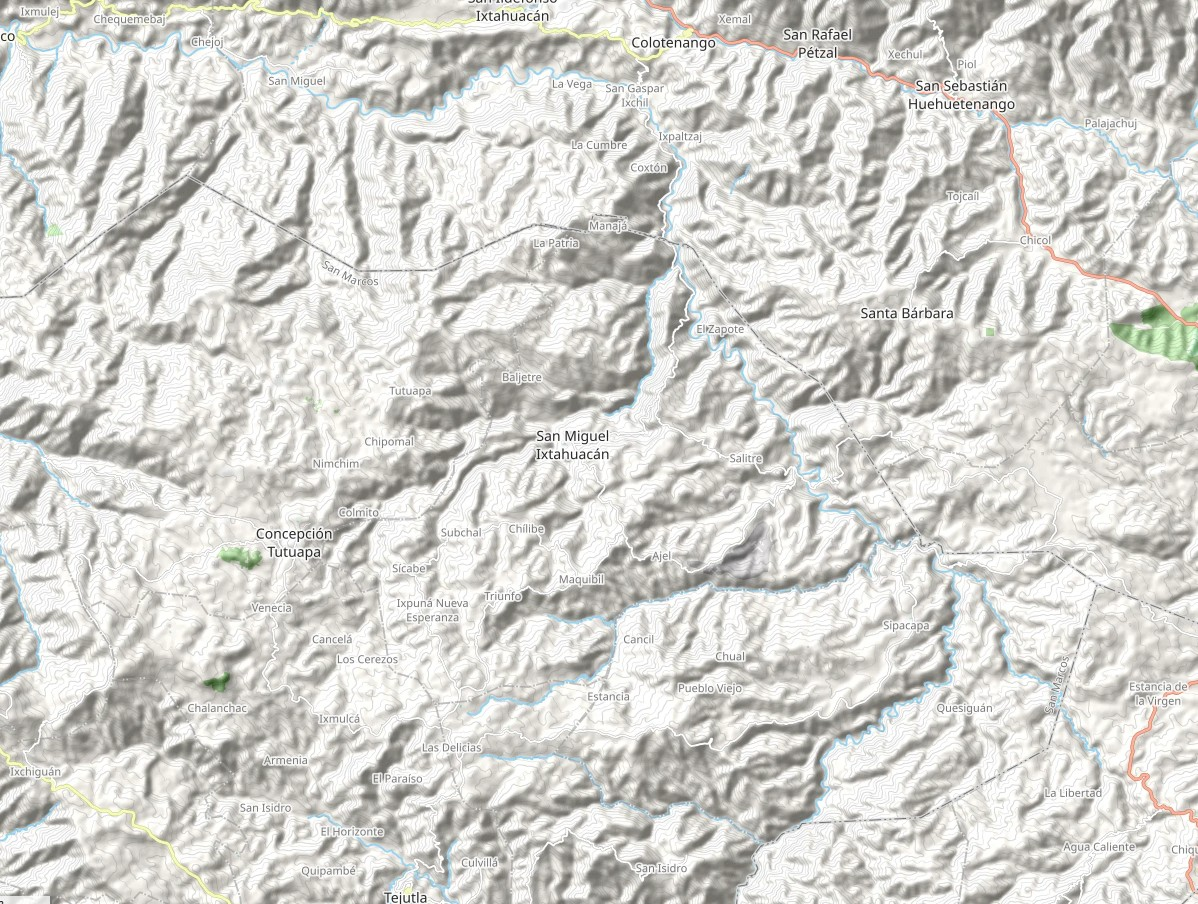
\includegraphics[width=0.85\textwidth]{imagenes/mapas/mapa_ubicacion_marlin.png}
%  \caption{Ubicación de la Mina Marlin, departamento de San Marcos, Guatemala}
%  \label{fig:mapa-ubicacion}
%  \par\vspace{2pt}
%  \raggedright\footnotesize Nota. Mapa base de OpenStreetMap,
%  \textcopyright{} OpenStreetMap contributors, licencia ODbL
%  \parencite{osmsfmapa}. Coordenadas del yacimiento:
%  15\textdegree14\textquotesingle05\textquotedbl{} N,
%  91\textdegree41\textquotesingle22\textquotedbl{} O.
%\end{figure}

% ---------------------------------------------------------------------
\subsection{Entorno social y económico}

La población de los municipios de San Miguel Ixtahuacán y Sipacapa asciende
conjuntamente a unos 70.000 habitantes y es mayoritariamente indígena: maya-mam
en San Miguel Ixtahuacán y maya-sipakapense en Sipacapa. La base económica
predominante es la agricultura de subsistencia
\parencite{oncommonground2010hria, ocmalsfmarlin}.

Este párrafo, breve en extensión, es el que sostiene toda la dimensión social del
informe y conviene explicitar por qué. Que el territorio afectado esté habitado
por pueblos indígenas no constituye un dato demográfico accesorio: es el hecho
jurídico que activa el Convenio 169 de la Organización Internacional del Trabajo
y el Performance Standard 7 de la Corporación Financiera Internacional, expuestos
ambos en la sección \ref{sec:marco} \parencite{oit1989convenio169}. Sin esa
condición, la ausencia de consulta previa sería una deficiencia de
relacionamiento comunitario; con ella, se convierte en el incumplimiento de una
obligación internacional exigible, que es exactamente como se clasifica en la
sección \ref{sec:hallazgos}.

A ello se añade un segundo factor, de naturaleza económica. Una población de
agricultura de subsistencia mantiene con el territorio una relación de dependencia
material directa: la tierra y el agua no son un entorno, son el medio de vida. La
consecuencia es que el umbral a partir del cual un impacto ambiental se percibe
como una amenaza existencial es mucho más bajo que en un entorno urbano o
industrializado. Esta asimetría en la percepción del riesgo, más que la magnitud
absoluta de los impactos medidos, explica buena parte de la persistencia del
conflicto y del desencuentro entre los monitoreos oficiales y la experiencia
comunitaria que se discute en la sección \ref{sec:critico}.

% ---------------------------------------------------------------------
\subsection{Marco geológico y mineralización}

La Mina Marlin explotó oro (Au) como producto principal y plata (Ag) como
coproducto de valor económico relevante. El yacimiento corresponde a un depósito
\textbf{epitermal de baja sulfuración de Au-Ag}, controlado estructuralmente por
la falla Virginia. La roca huésped está constituida por una unidad volcánica
máfica de edad terciaria y por tobas andesíticas pertenecientes al denominado
Complejo Marlin \parencite{sec2011ni43101}.

La mineralización se presenta en forma de vetas y de \textit{stockworks} de cuarzo
bandeado, calcita y adularia. La asociación mineralógica documentada incluye
pirita, acantita, pirargirita-proustita, y oro nativo y electrum. Esta composición
tiene una implicación ambiental que conviene señalar desde ahora: la presencia
significativa de pirita en la roca huésped y en el desmonte es la condición
geoquímica que genera el potencial de \textbf{drenaje ácido de roca}. Al quedar
expuesta la pirita a la acción del oxígeno y el agua, su oxidación produce
acidez, que a su vez moviliza metales pesados hacia las aguas superficiales y
subterráneas. El riesgo de drenaje ácido identificado por la auditoría no es, por
tanto, una contingencia operativa: es una consecuencia previsible de la geología
del yacimiento, y como tal debía haber sido anticipada desde el estudio de
impacto ambiental \parencite{moran2004review}.

Las estructuras mineralizadas se agrupan en varias vetas y zonas. La veta Virginia
concentró la producción subterránea histórica; junto a ella se reconocen las vetas
Rosa y Tello-Tomates. En el ámbito del tajo abierto se explotaron la zona Marlin
o \textit{Main Zone}, West Vero y La Hamaca, además del tajo satélite Cochis
\parencite{sec2011ni43101}.

La Tabla \ref{tab:reservas} resume las reservas y los recursos declarados en el
informe técnico NI 43-101. Debe leerse con una precaución metodológica: las
reservas no son una propiedad permanente del yacimiento, sino una estimación
referida a una fecha y a unos supuestos económicos determinados. Los valores que
se consignan tienen fecha efectiva de 31 de diciembre de 2010, es decir,
corresponden a la mitad de la vida útil de la operación y no a su totalidad.

% --- TABLA: Reservas y recursos --------------------------------------
\begin{table}[H]
  \centering
  \caption{Reservas y recursos declarados de la Mina Marlin (fecha efectiva: 31 de diciembre de 2010)}
  \label{tab:reservas}
  % \small y un \tabcolsep reducido: con seis columnas y cifras de ocho
  % dígitos, a tamaño normal la tabla se sale del margen.
  \begin{small}
  \setlength{\tabcolsep}{5pt}
  \begin{tabular}{@{}l r r r r r@{}}
    \toprule
    \textbf{Categoría} & \textbf{Tonelaje} & \textbf{Ley Au} & \textbf{Ley Ag}
      & \textbf{Au contenido} & \textbf{Ag contenida} \\
     & \textbf{(kt)} & \textbf{(\gt)} & \textbf{(\gt)}
      & \textbf{(\ozAu)} & \textbf{(\ozAg)} \\
    \midrule
    Reservas probadas y probables & 9.211 & 5,17 & 203,6 & 1.529.600 & 60.296.200 \\
    Recursos medidos e indicados\textsuperscript{a} & 922 & 1,78 & 78,8 & --- & --- \\
    \bottomrule
  \end{tabular}
  \end{small}
  \par\vspace{3pt}
  \raggedright\footnotesize
  Nota. \textsuperscript{a}Exclusivos de reservas. El informe técnico no reporta
  el contenido de metal de esta categoría; los guiones indican dato no
  disponible en la fuente, no ausencia de contenido metálico. Tomado de
  \textcite{sec2011ni43101}.
\end{table}
% NOTA PARA QUIEN EDITE: si quieres rellenar las dos celdas con «---», puedes
% calcularlas (tonelaje x ley / 31,1035 g por onza troy), pero DEBES indicar en
% la nota que son valores calculados y no tomados del informe técnico.

% ---------------------------------------------------------------------
\subsection{Método de explotación}

La Mina Marlin operó mediante un \textbf{método mixto}, combinando explotación a
tajo abierto y explotación subterránea. El tajo se desarrolló mediante bancos y
terrazas concéntricas, conforme a la configuración habitual en yacimientos de
este tipo. La explotación subterránea se realizó mediante una rampa en espiral de
4,6 m de ancho por 4,9 m de alto; hacia el final de la vida útil de la operación
se habían desarrollado aproximadamente 147 km de labores subterráneas
\parencite{sec2011ni43101}.

La coexistencia de ambos métodos generó dos perfiles de impacto claramente
diferenciados, y conviene distinguirlos porque las quejas comunitarias
documentadas en la auditoría se dirigen a uno y otro por separado.

El tajo abierto produce impactos de superficie: remoción de cobertura vegetal y
suelo, alteración del relieve, generación de grandes volúmenes de desmonte —con
el consiguiente potencial de drenaje ácido ya señalado—, emisión de material
particulado y vibraciones por voladura. Son impactos visibles, medibles y
relativamente fáciles de atribuir.

La explotación subterránea, en cambio, produce impactos menos evidentes pero de
atribución más disputada: subsidencia, alteración de los niveles freáticos y
vibraciones transmitidas por el macizo rocoso. El agrietamiento de viviendas en
las comunidades del entorno constituyó uno de los motivos de queja recurrentes de
la población, y es un caso ilustrativo de la dificultad probatoria que atraviesa
todo el expediente: establecer si una grieta obedece a la actividad minera, a la
sismicidad regional o a la calidad constructiva de la vivienda exige una línea
base y un monitoreo estructural previos que, de no existir, hacen la controversia
técnicamente irresoluble \parencite{oncommonground2010hria}. Este punto anticipa
uno de los ejes del análisis crítico de la sección \ref{sec:critico}: la ausencia
de línea base robusta no es un detalle técnico, sino la condición que perpetúa el
desacuerdo.

% ---------------------------------------------------------------------
\subsection{Procesamiento metalúrgico}

El circuito de beneficio empleado en Marlin corresponde al esquema convencional de
recuperación de oro y plata por cianuración, con recuperación final por
precipitación con zinc. La secuencia documentada es la siguiente
\parencite{sec2011ni43101}:

\begin{enumerate}
  \item \textbf{Trituración.} Reducción granulométrica primaria del mineral
        procedente del tajo y de la mina subterránea.
  \item \textbf{Molienda.} Molino SAG seguido de molino de bolas, hasta alcanzar
        una granulometría de 85 \% pasante la malla 200.
  \item \textbf{Lixiviación por agitación con cianuro}, en configuración de tipo
        CIL (\textit{carbon in leach}), en la que la disolución del oro y la plata
        y su adsorción sobre carbón activado ocurren simultáneamente.
  \item \textbf{Decantación en contracorriente}, para la separación y el lavado
        de la solución rica respecto de los sólidos.
  \item \textbf{Precipitación Merrill-Crowe con zinc}, que recupera los metales
        preciosos de la solución mediante cementación.
  \item \textbf{Fundición}, con obtención de barras doré de oro y plata como
        producto final comercializable.
  \item \textbf{Destrucción de cianuro} mediante el proceso INCO, aplicado a la
        pulpa antes de su depósito en la instalación de relaves.
\end{enumerate}

Dos aspectos de este circuito merecen comentario desde la perspectiva de la
auditoría. El primero es que el uso de cianuro constituye el aspecto ambiental
más significativo de toda la operación, en el sentido técnico que la
ISO 14001:2015 da a ese término y que se definió en la sección \ref{sec:marco}.
El segundo es que la operación incorporó un circuito específico de destrucción de
cianuro previo al depósito de relaves, y que fue la primera mina de Centroamérica
certificada bajo el \textit{International Cyanide Management Code}. Este dato es
relevante y debe consignarse con exactitud: acredita la adopción de un estándar
internacional voluntario en materia de manejo de cianuro, pero no equivale a una
certificación del desempeño ambiental global de la operación ni cubre los
riesgos de drenaje ácido, que tienen un origen geoquímico distinto y quedan fuera
del alcance de ese código. Confundir ambas cosas —una certificación específica
con una garantía general— es precisamente el tipo de inferencia que una auditoría
debe evitar.

% --- FIGURA 2: Diagrama de flujo del proceso -------------------------
% PENDIENTE DE INSERTAR. Puedes dibujarlo en TikZ o hacerlo en draw.io /
% PowerPoint y exportarlo a PDF (NO a JPG). Guárdalo en imagenes/diagramas/.
% Sigue la secuencia de los siete pasos enumerados arriba.
%\begin{figure}[H]
%  \centering
%  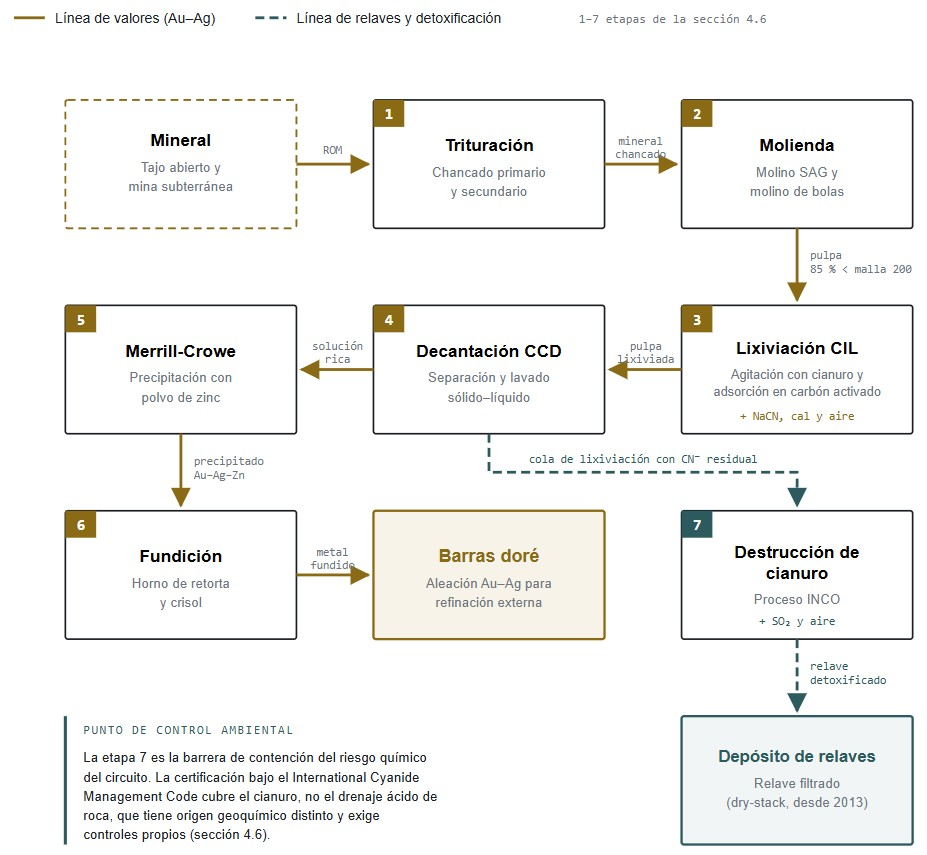
\includegraphics[width=0.9\textwidth]{imagenes/diagramas/flujo_proceso.pdf}
%  \caption{Diagrama de flujo del proceso metalúrgico de la Mina Marlin}
%  \label{fig:flujo-proceso}
%  \par\vspace{2pt}
%  \raggedright\footnotesize Nota. Elaboración propia a partir de
%  \textcite{sec2011ni43101}.
%\end{figure}

% ---------------------------------------------------------------------
\subsection{Capacidad de tratamiento: precisión sobre las cifras}

La capacidad de tratamiento de la planta es uno de los datos que con mayor
frecuencia aparece distorsionado en las fuentes secundarias sobre este caso, y su
tratamiento riguroso constituye en sí mismo un ejercicio de auditoría. No existe
una cifra única correcta: existen varias métricas distintas, cada una válida en
su propio marco, que solo pueden compararse si se declara a qué se refiere cada
una. La Tabla \ref{tab:capacidad} las presenta de forma explícita.

% --- TABLA: Capacidad de tratamiento ---------------------------------
\begin{table}[H]
  \centering
  \caption{Capacidad de tratamiento de la planta de la Mina Marlin según la métrica declarada}
  \label{tab:capacidad}
  \begin{tabularx}{\textwidth}{@{}L{4.3cm} L{3.3cm} Y@{}}
    \toprule
    \textbf{Métrica} & \textbf{Valor} & \textbf{Observación} \\
    \midrule
    Diseño nominal del molino & $\approx$1,82 Mt/año & Capacidad de diseño original. \\
    \addlinespace
    Capacidad optimizada & $\approx$2,05 Mt/año \newline ($\approx$5.000--5.600 \tdia) &
      Tras las mejoras introducidas en el circuito. \\
    \addlinespace
    Procesamiento real (2010) & $\approx$1,4 Mt/año \newline ($\approx$3.800 \tdia) &
      Tratamiento efectivo, inferior a la capacidad instalada. \\
    \addlinespace
    Rango operativo declarado en la venta de la planta & 4.000--7.000 \tdia \newline
      (promedio $\approx$6.000 \tdia) & Cifra del anuncio de venta del activo;
      procede de una fuente comercial, no técnica. \\
    \midrule
    \multicolumn{3}{@{}l}{\textit{Dato que NO corresponde a capacidad de planta:}} \\
    Material total minado & $\approx$24.282 \tdia &
      Incluye mineral \textbf{y} desmonte. No es capacidad de tratamiento. \\
    \bottomrule
  \end{tabularx}
  \par\vspace{3pt}
  \raggedright\footnotesize
  Nota. Elaboración propia a partir de \textcite{sec2011ni43101} y
  \textcite{miningcomsfventa}.
\end{table}

La distinción de la última fila es la más importante y la que con más frecuencia
se pasa por alto. La cifra aproximada de 24.282 \tdia\ que figura en el informe
técnico corresponde al \textbf{material total minado}, esto es, la suma del
mineral enviado a planta y del desmonte movido para acceder a él. Presentarla
como capacidad de tratamiento supone multiplicar por un factor de entre cuatro y
seis la capacidad real de la planta. Un informe de auditoría que incurriera en
esa confusión perdería credibilidad técnica en su conjunto, y por eso se deja
constancia expresa del punto.

Debe señalarse asimismo que la cuarta fila procede de un anuncio comercial de
venta del activo, no de un documento técnico sometido a estándar de reporte. Se
incluye por transparencia y porque es la fuente que sostiene las cifras más altas
que circulan sobre la operación, pero su jerarquía probatoria es inferior a la
del informe NI 43-101 y así debe ponderarse.

% ---------------------------------------------------------------------
\subsection{Producción, empleo y ciclo de vida de la operación}

A lo largo de sus doce años de operación, entre 2005 y 2017, la Mina Marlin
produjo \textbf{2,3 millones de onzas de oro y 63 millones de onzas de plata},
cifra confirmada por la propia empresa \parencite{goldcorp2017legacy}. Ello
equivale a un promedio anual del orden de 250.000 \ozAu\ y 3,5 millones de
\ozAg. La operación fue la mayor mina y la principal exportadora de oro de
Guatemala y de Centroamérica.

En cuanto al empleo, la operación alcanzó un máximo aproximado de 3.000
trabajadores en su fase de mayor actividad. En operación plena se estimaban
alrededor de 2.000 empleos directos y unos 8.000 indirectos. Al momento del
cierre, la plantilla se había reducido a unos 1.200 trabajadores
\parencite{oncommonground2010hria, prensalibre2017cierre}.

Estas magnitudes conviene interpretarlas, no solo enunciarlas. El eje de
inversión económica y social de la auditoría reconoció que la operación generó
aportes efectivos en empleo e ingresos, y las cifras anteriores lo confirman. Pero
el mismo eje concluyó que la mitigación de los impactos negativos resultó
insuficiente. Ambas afirmaciones son compatibles y su coexistencia es
precisamente el núcleo del problema: la magnitud del beneficio agregado no
compensa automáticamente la distribución desigual de los perjuicios, sobre todo
cuando beneficios y perjuicios recaen sobre poblaciones distintas y en horizontes
temporales distintos. El empleo dura lo que dura la mina —doce años— mientras que
el pasivo ambiental permanece indefinidamente. Esta asimetría temporal es la que
convierte la planificación del cierre y del post-cierre, tratada en la sección
\ref{sec:plan}, en la cuestión decisiva del caso.

El cierre de producción se produjo el 31 de mayo de 2017 e incluyó un plan de
recuperación ambiental con destrucción de cianuro y relleno del tajo
\parencite{goldcorp2023marlin}. Que la operación haya completado su ciclo
íntegro —construcción, operación, conflicto, auditoría, plan de acción, cierre y
post-cierre— es lo que permite a este informe evaluar la mejora continua sobre un
caso cerrado y no sobre una operación todavía en curso.

% ---------------------------------------------------------------------
\subsection{Infraestructura crítica y gestión de relaves}

La instalación de mayor criticidad ambiental de la operación fue el depósito de
relaves (\textit{tailings storage facility}), construido entre 2004 y 2010 en el
valle situado al norte de la planta de proceso. Con posterioridad, la operación
inició la transición hacia un esquema de relaves filtrados o apilamiento en seco
(\textit{dry-stack}), mediante una planta de filtrado de marca Metso instalada en
2013 y operativa hasta el cierre en 2017 \parencite{sec2011ni43101}.

Esta transición merece una valoración positiva explícita, porque constituye uno de
los pocos elementos del expediente en que la operación se adelantó a la evolución
del estándar sectorial. El apilamiento en seco reduce sustancialmente el riesgo
de rotura catastrófica al eliminar el embalse de agua que caracteriza a los
depósitos convencionales, que es precisamente el mecanismo que produjo los
colapsos de Mount Polley, Samarco y Brumadinho. Que Marlin iniciara esa
transición en 2013 —seis años antes de Brumadinho y siete antes de la publicación
del Global Industry Standard on Tailings Management— es un dato que el análisis
debe reconocer con la misma objetividad con que consigna las deficiencias
\parencite{icmm2020gistm}.

La operación contó además con una planta de tratamiento de agua, puesta en
servicio en 2008, y con un aliviadero de emergencia dimensionado para la Crecida
Máxima Probable, cuya construcción supuso una inversión aproximada de US\$ 14
millones y más de 8.000 m\textsuperscript{3} de concreto. En materia de
verificación, el depósito fue objeto de revisiones quinquenales de seguridad de
presa conforme a los protocolos de la Canadian Dam Association, realizadas por
Tierra Group International \parencite{sec2011ni43101}.

\subsubsection{Limitación de información declarada}

Es preciso dejar constancia expresa de una limitación en la información
disponible. No fue posible verificar, en fuente primaria específica de la Mina
Marlin, tres parámetros básicos del depósito de relaves: el \textbf{tipo
constructivo de la presa} —aguas arriba, aguas abajo o de línea central—, su
\textbf{altura} y su \textbf{volumen almacenado}. Estos datos requerirían el
acceso al estudio de impacto ambiental detallado o al informe de diseño de
ingeniería de la instalación.

La omisión es deliberada y conviene justificarla, porque un lector podría
interpretarla como una laguna de la investigación. En primer lugar, el método
constructivo de una presa de relaves es el parámetro que más determina su perfil
de riesgo: fue el método aguas arriba el que falló por licuefacción estática en
Brumadinho \parencite{robertson2019feijao}. Atribuir a Marlin un método
constructivo no verificado sería, por tanto, comprometer el hallazgo más sensible
del análisis sobre la base de una conjetura. En segundo lugar, sobre este caso
circulan en fuentes secundarias cifras que corresponden en realidad a otras
operaciones mineras, de modo que el riesgo de contaminación de datos es real y
documentado. Declarar la limitación es metodológicamente preferible a rellenarla
con una cifra plausible: en auditoría, la ausencia de evidencia se registra como
tal y no se sustituye por inferencia.

Finalmente, cabe señalar que durante el período de operación no existía todavía un
estándar internacional específico y auditable para la gestión de relaves. El
GISTM se publicó en 2020, tres años después del cierre. La gestión del depósito se
verificaba, en consecuencia, contra protocolos privados y guías nacionales de
terceros países, como los de la Canadian Dam Association ya mencionados. Esta
circunstancia debe tenerse presente al valorar los hallazgos ambientales de la
sección \ref{sec:hallazgos}: la vara de medir disponible en su momento era
sustancialmente menos exigente que la actual, lo que no exime de responsabilidad
pero sí obliga a evaluar la conducta contra los criterios vigentes entonces y no
contra los de hoy.
